\documentclass[tikz,border=2pt]{standalone}
\usepackage{amsmath,amssymb}
\usepackage{pgfplots}
\pgfplotsset{compat=1.18}

\begin{document}
% The saddle f = x_1^2 - x_2^2 at the origin: the gradient vanishes, yet f rises along the
% x_1-axis and falls along the x_2-axis, so the point is neither a maximum nor a minimum.
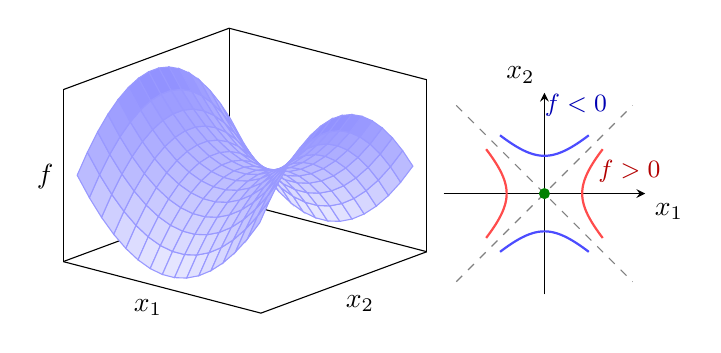
\begin{tikzpicture}
	\begin{axis}[name=p1, view={40}{25}, xmin=-1.3, xmax=1.3, ymin=-1.3, ymax=1.3, zmin=-1.6, zmax=1.6, xlabel={$x_1$}, ylabel={$x_2$}, zlabel={$f$}, zlabel style={rotate=-90}, xtick=\empty, ytick=\empty, ztick=\empty, width=6.2cm, height=5.2cm]
		\addplot3[surf, shader=faceted, faceted color=blue!40, colormap={pale}{color=(blue!8) color=(blue!45)}, samples=16, domain=-1.2:1.2, domain y=-1.2:1.2, z buffer=sort] {x^2-y^2};
	\end{axis}
	\begin{axis}[name=p2, at={(p1.outer east)}, anchor=outer west, xshift=0.2cm, axis lines=middle, axis equal image, xmin=-1.6, xmax=1.6, ymin=-1.6, ymax=1.6, xtick=\empty, ytick=\empty, xlabel={$x_1$}, ylabel={$x_2$}, xlabel style={below right}, ylabel style={above left}, samples=60, clip=false, width=4.8cm]
		\addplot[red!70, thick, domain=-1.0:1.0] ({0.6*cosh(x)}, {0.6*sinh(x)});
		\addplot[red!70, thick, domain=-1.0:1.0] ({-0.6*cosh(x)}, {0.6*sinh(x)});
		\addplot[blue!70, thick, domain=-1.0:1.0] ({0.6*sinh(x)}, {0.6*cosh(x)});
		\addplot[blue!70, thick, domain=-1.0:1.0] ({0.6*sinh(x)}, {-0.6*cosh(x)});
		\addplot[gray, dashed, domain=-1.4:1.4, samples=2] {x};
		\addplot[gray, dashed, domain=-1.4:1.4, samples=2] {-x};
		\fill[green!50!black] (axis cs:0,0) circle (2pt);
		\node[red!70!black, font=\small] at (axis cs:1.35,0.35) {$f>0$};
		\node[blue!70!black, font=\small] at (axis cs:0.5,1.4) {$f<0$};
	\end{axis}
\end{tikzpicture}
\end{document}
